\section{System}
\label{sec:system}
\subsection{Data, degradation and visual odometry}
All studies use TartanGround \cite{tartanground} (RENDERED, CC BY 4.0 \cite{tg_hf}), the first 200 s of each trajectory, the front stereo pair at 320 by 320 pixels, and the frozen Study~2 degradation (Koschmieder dust haze along depth \cite{cheng}, low light with exposure and noise, motion blur, glare, frame drops; levels D0 to D4 with visibility none, 1000, 200, 60 and 20 m) and stereo visual odometry (KLT tracking, PnP with RANSAC, no mapping). Fig.~\ref{fig:frames} shows the levels. The IMU is the noise free dataset IMU with added noise and bias random walks.

\begin{figure*}[t]
\centering
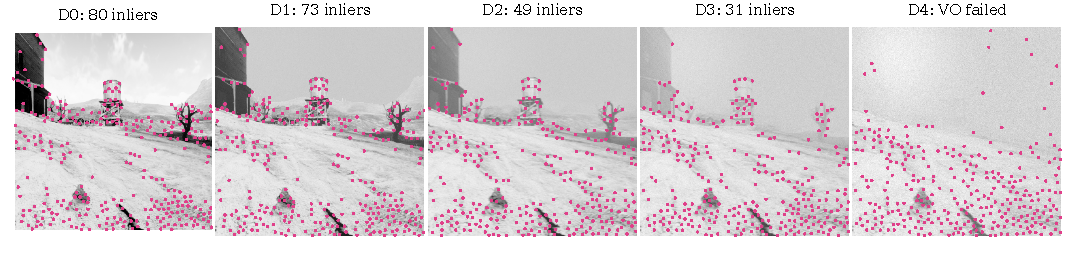
\includegraphics[width=0.9\textwidth]{figs/fig_frames.pdf}
\caption{One pilot frame at levels D0 to D4 (RENDERED image, SIMULATED degradation) with tracked features and PnP inliers.}
\label{fig:frames}
\end{figure*}

\subsection{Filter}
A ten state extended Kalman filter estimates planar position, yaw, world velocity, gyro bias, two accelerometer biases, a compass heading bias and a visual forward speed scale error. The two new states are inert (zero variance) unless a system uses them, and a unit test checks that the filter then reproduces the Study~2 filter exactly. The IMU drives the prediction at 100 Hz; visual odometry updates body velocity and gyro bias at 10 Hz with bounded inflation of outliers; the compass updates yaw at 5 Hz.

\subsection{Systems}
Table~\ref{tab:systems} lists the nineteen systems. B0 to B3 are the earlier baselines with their frozen parameters. B4 (DoP floor for covariance matching, no gate) was exploratory in Study~2 and is tested here. B5 to B8 are new weighting schemes; one of them, S, is selected on the development split by a written rule. B3L adds a lock out recovery rule, B3C the calibrated noise model fitted on the pilot split (a Gauss Markov visual speed scale with $\sigma = \sPilotSv{}$ and $\tau = \sPilotTau{}$ s, and the variance of the averaged gyro in the bias measurement, which the earlier filter omitted). B3R and B4R use the zenith and ring geometry, SUN and MAG a sun sensor and a magnetometer with assumed error models. W0, W3 and W4R replace the camera with simulated wheel odometry (scale error 2 percent, white noise 0.05 m/s, slip epochs that add 15 percent).

\begin{table}[t]
\caption{Study 3 systems (one filter, different compass and odometry inputs).}
\label{tab:systems}
\centering\footnotesize\setlength{\tabcolsep}{3pt}
\begin{tabular}{ll}
\toprule
ID & Compass update and odometry \\
\midrule
B0 & none; stereo VO in all B and S systems \\
B1, B1g & fixed 1 degree, without and with a $\chi^2$ gate (6.63) \\
B2 & covariance matching, window 3, floor 1 degree \\
B3 & noise from measured DoP, gate \\
B4 & DoP noise as floor of covariance matching, no gate \\
B5 & two mode (good, 45 degree bad) moment matched IMM \\
B6 & Huber weighting ($k = 1.345$) of the DoP noise \\
B7 & B3 with a compass bias state \\
B8 & learned reliability (logistic, pilot split) \\
B3L & B3 with lock out recovery after 5 s \\
B3C & B3 with the calibrated (coloured) noise model \\
B3R, B4R & B3, B4 with the zenith and ring geometry \\
SUN, MAG & sun sensor, magnetometer (ASSUMED) \\
W0, W3, W4R & wheel odometry with no, zenith or ring compass \\
\bottomrule
\end{tabular}
\end{table}

\section{Protocol}
\label{sec:protocol}
Protocol v0.3 was frozen in a repository tag (commit faa2131) before any estimator ran on the confirmation split. It defines three splits. The pilot split (WesternDesertTown, 6 trajectories) fits the B8 model and the B3C noise model. The development split is the Study~2 held out set (34 trajectories in DesertGasStation, MiddleEast and EndofTheWorld), demoted because it has been inspected; it is used only to select S. The confirmation split is \sNconf{} trajectories from three environments never processed before (Ruins, AncientTowns and HQWesternSaloon), chosen by name before any image was viewed, with three degradation seeds at D2 and D4 and one at D0. Each visual odometry run is filtered under 16 scenarios (21 March, June, September and December; 09:30, 11:45, 12:30 and 14:30) with their own aerosol and cloud draws, and two IMU draws.

\textbf{Analysis.} The unit is the trajectory, averaged over levels D0, D2 and D4 unless a hypothesis names a level. Paired differences are summarised by their median with a two stage cluster bootstrap (environments, then trajectories, 10,000 resamples) and tested by a paired Wilcoxon signed rank test, one sided, with Holm correction over the superiority tests H1, H2, H4 and H5 (the protocol listed H1 to H6 in one section and excluded H6 in another; the non inferiority tests are decided by their intervals). Non inferiority uses a margin of 0.5 degrees on the upper bound of the 95 percent interval.

\textbf{Hypotheses.} H1: B3 has a lower heading RMSE than B0. H2: with bias (and tilt, see Section~\ref{sec:deviations}), the ungated B1 has a higher heading RMSE than B0 at D0. H3: S is not worse than B2 (margin 0.5 degrees). H3b: B4 is not worse than B2 (same margin). Because the development rule selected S = B4, H3 and H3b reduce to the same comparison. H4: the ring geometry (B4R) has a lower heading RMSE than the zenith point (B4). H5: wheel odometry with the compass (W3) has a lower drift than stereo VO without it (B0) at D4. Criterion checks outside the family: H6, B3C has a median position NEES in [1, 4] and a mean 95 percent coverage in [0.8, 0.99]; H7, the development and confirmation rankings of the VO systems agree with Kendall $\tau \ge 0.6$. The blind window results above were computed before the freeze and are model results, not confirmatory tests.
